\chapter{Deep Learning Models for Fetal Pain Assessment}

Based on the techniques mentioned in Chapter 3, we have proposed a process and a few learning models for classifying images of fetuses with facial expressions containing the presence of pain or not. In summary, our proposed pipeline consists of sampling the videos into frames, finding the images which contain a clear fetus face, and training a Convolutional Neural Network (CNN), with the help of transfer learning, for the binary classification task of finding the presence of pain. In the following sections, we describe each of these steps.

\section{Image Sampling}

It is common to have a small number of data to work within the medical field in general, given the inherent difficulty of collecting it \citep{abs-1908-00473}. In our case, especially, only a small percentage of pregnancies require intra-uterus intervention before birth, and thus fetal anesthesia is a relatively rare procedure. Thus, as seen in the previous chapter, we ended up with 13 videos available, which is a number similar to what we have seen in other studies, such as the iCOPE database.

Since we had a small number of videos, it was not possible to work with them directly. So, we brought the data to another dimension, reducing the space from videos to images by sampling them and capturing frames at a rate of every 2 seconds. 

With this process, we generated a total of 708 images, but since the images were recorded from ultrasound machines, they depend on the calibration by the specialists to capture the exact section of the 3-D space where the fetus's face is clear. Because of this, it was common to find parts of the video where the face of the fetus was not visible and showed non-distinguishable parts. As we had a significant number of images, and manual selection would be not only hard but also dependent on the observant, this became a problem.

To overcome this issue, we decided to use another neural network capable of detecting facial landmarks, like the nose, the mouth, and the eyes. The network we used was the Multi-task Cascaded Convolutional Networks (MTCNN) developed by \cite{ZhangZL016}, which is trained to identify faces in images. It worked surprisingly well in our domain, even though the images had quite different characteristics.

With this process, we were able to filter our dataset and reduce the number of images from 708 to 357, but being sure the images contained a clear face. The network also returns a confidence value of which it found the face in the image, and we have used only confidences of over 95\%, which, after manual inspection, showed to be very reliable, with just six clear errors that were removed manually.

The position of the facial landmarks encountered by the network also allowed us to crop images around the fetus's face. This process is achievable after we have the coordinates of the landmarks returned through the MTCNN, which also makes face alignment possible. This helps to discard images with blurred surroundings around the fetus, which contains non-distinguishable parts. In Figure \ref{fig:cropping}, we can see an example of a sampled image and its respective cropping.

\begin{figure}[h!tp]
    \centering
    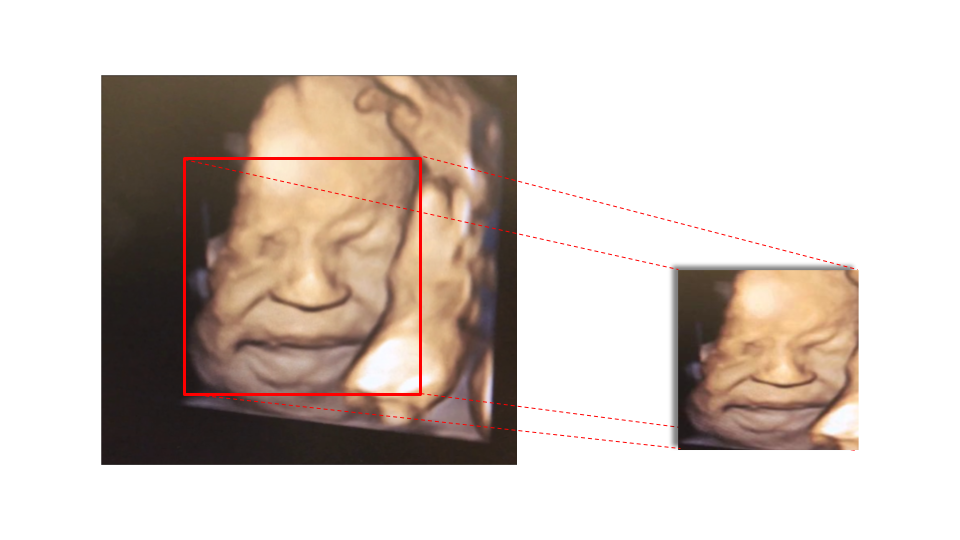
\includegraphics[width=.7\textwidth]{imgs/chap5_cropping.png}
    \caption{Image cropping with MTCNN}
    \label{fig:cropping}
\end{figure}

In the videos of acute pain, as we knew precisely when the anesthetic puncture stimuli were applied, it was possible to divide the images into the two classes of pain and non-pain. This division is relevant, as it allows us to experiment in the scenario where we can evaluate the same fetus, for both conditions. In the other two groups, this is not possible as we have only images of the non-pain class.

\section{Data Augmentation}

Even though we had increased the size of the dataset by turning the videos into images, it is still considered a relatively small dataset for deep learning models. To further augment our chances of succeeding, we have applied the use of data augmentation techniques to increase the variability of our data. The effectiveness of this technique has been demonstrated by \cite{abs-1712-04621} and is widely used in the field.

There is a wide variety of transformations possible for using data augmentation, and even simple techniques already work very well. We have chosen to apply the following transformations:

\begin{itemize}
    \item Horizontal flip, which mirrors the image horizontally. 
    \item Rotation, which applies rotations to the images up to a maximum degree.
    \item Zooming, which zooms into parts of the image up to a maximum level.
    \item Warping, which adds distortions to the image up to a maximum level.
    \item Lighting, which changes the brightness and the contrast of the images.
\end{itemize}

All of these methods have a probability of being applied and can be used in combination with each other. Thus for each image, given the probability, a combination of these techniques would be applied. Some examples of these different combinations within the same image are shown in Figure \ref{fig:data_augmentation}.

\begin{figure}[h!tp]
    \centering
    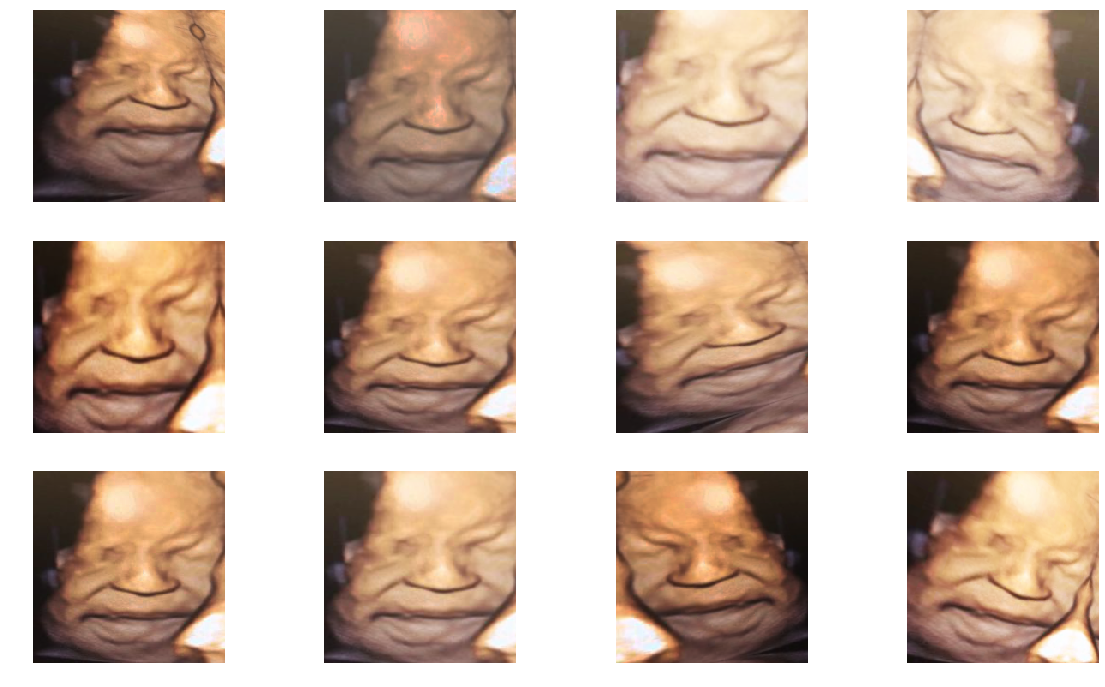
\includegraphics[width=.75\textwidth]{imgs/chap5_data_augmentation.png}
    \caption{Application of different data transformations to a fetus image}
    \label{fig:data_augmentation}
\end{figure}

To further experiment with this process, we have compared two levels of intensity in the changes regarding their max levels of rotation, zoom, warping, and lightning. First, a weak set of transformations, which does subtle changes in the images. Later, a stronger set, which applies substantial changes to the images.

\section{Residual Networks}

The network used was a ResNet created by \cite{ParkhiVZ15}.

\section{Transfer Learning}

When using transfer learning, the features computed in the early layers of the network usually are already well trained in doing basic tasks such as recognizing basic lines, patterns, or gradients. On the other hand, the features computed in the later layers are the ones highly dependent on the specific task we are trying to predict. Thus, when we are fine-tuning the network in our domain, we have two main approaches to train the network, namely with frozen or unfrozen layers. These methods allow us to decide which specific layers of our model we want to train at a given time. 

In the frozen approach, all layers except the last one will be untrainable. In the unfrozen approach, however, all the layers are kept unfrozen during training, and the errors are back-propagated to the entire network during fine-tuning. Hence, even the early layers may be affected. In our experiments, we decided to test both approaches, as even though unfreezing the layers appears to be better, we were unsure if the amount of data and its noise would be enough to improve the weights of the whole network.

VGGFace2: \citep{Cao2018}
ImageNet: \citep{DengDSLL009}


